%!TEX root = /Users/Daniel/Documents/Imperial/project/tevatron-higgs/report/report.tex

The performance of a neural network is highly dependent on both the number of nodes and the network topology. 
In theory by the Universal Approximation Theorem, an ANN with sufficiently many nodes arranged in single hidden layer is able to approximate an arbitrary decision boundary. However in practice deep neural networks can perform better, so a variety of sizes and topologies were investigated and evaluated. 

A commonly used criterion for measuring signal/background separation performance is the significance, $\frac{S(c)}{\sqrt{B(c)}}$ where $S(c)$ and $B(c)$ are the weighted number of signal and background events respectively, scoring above the signal acceptance cutoff $c$. Typically,  as a function of $ c \in (0,1)$, $\frac{S(c)}{\sqrt{B(c)}}$ has a maximum which can be used as a comparison.

Another evaluation parameter common in machine learning applications is the AUC, the area under the ROC (receiver operator characteristic) curve.
The ROC curve is the parametric plot of the true positive rate (tpr) against the false positive rate (fpr), parameterised by the cutoff.

\begin{figure}[h]
	\centering
	
	\begin{subfigure}{0.49\textwidth}
	      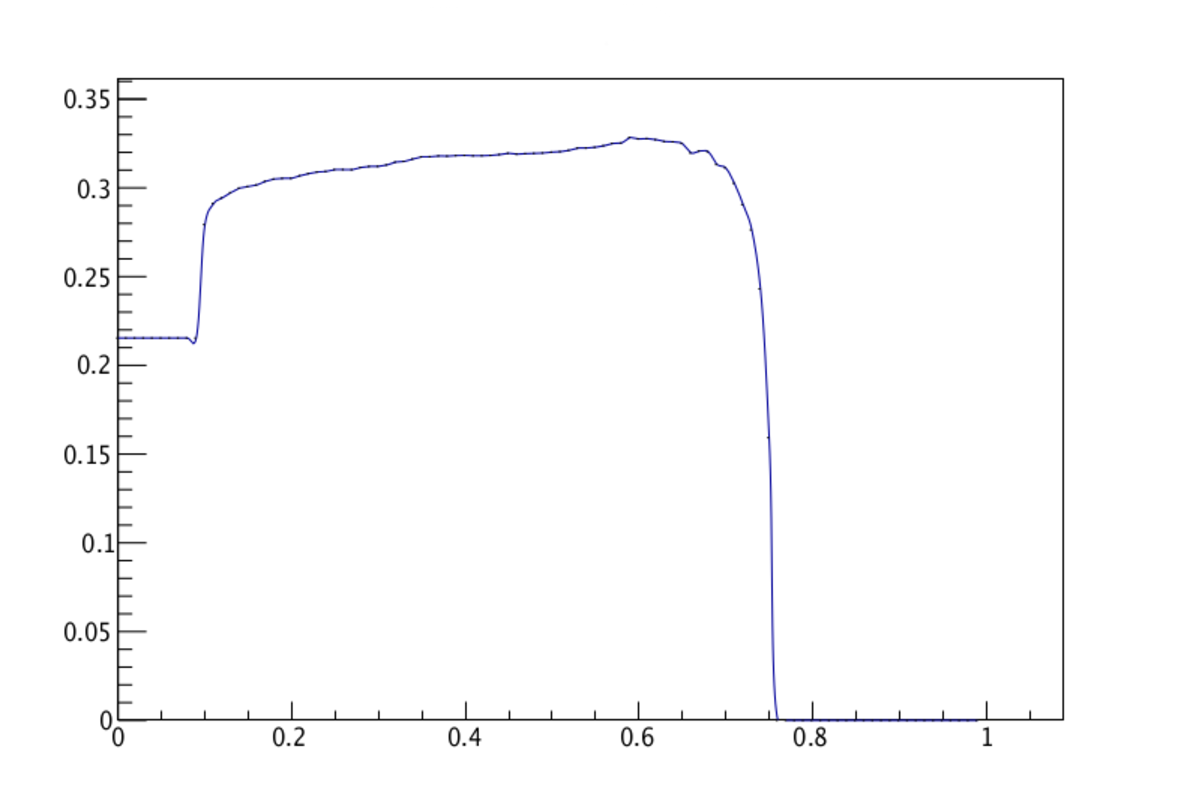
\includegraphics[width=\textwidth]{img/sig}
	      \caption{$\frac{S}{\sqrt{B}}$}
	\end{subfigure}
	\begin{subfigure}{0.49\textwidth}
	      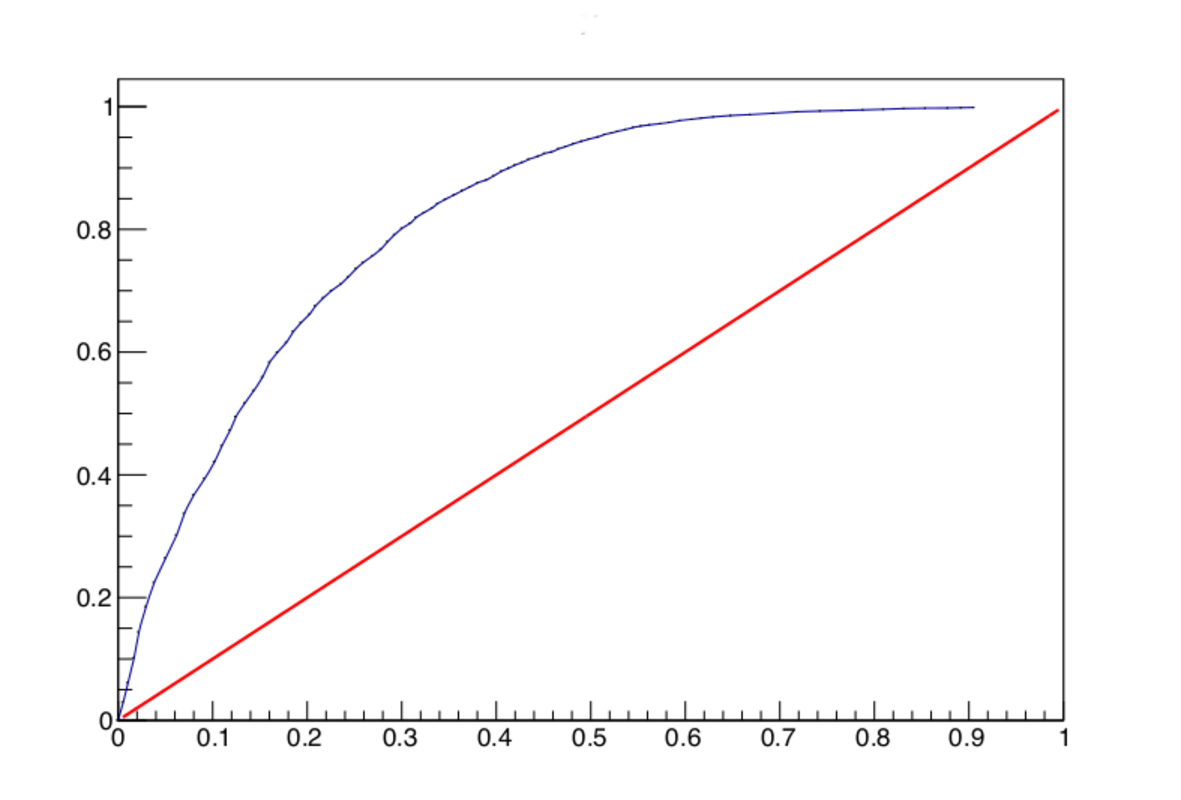
\includegraphics[width=\textwidth]{img/roc}
	      \caption{ROC curve of the classifier}
	\end{subfigure}
	
	\begin{subfigure}{0.5\textwidth}
	      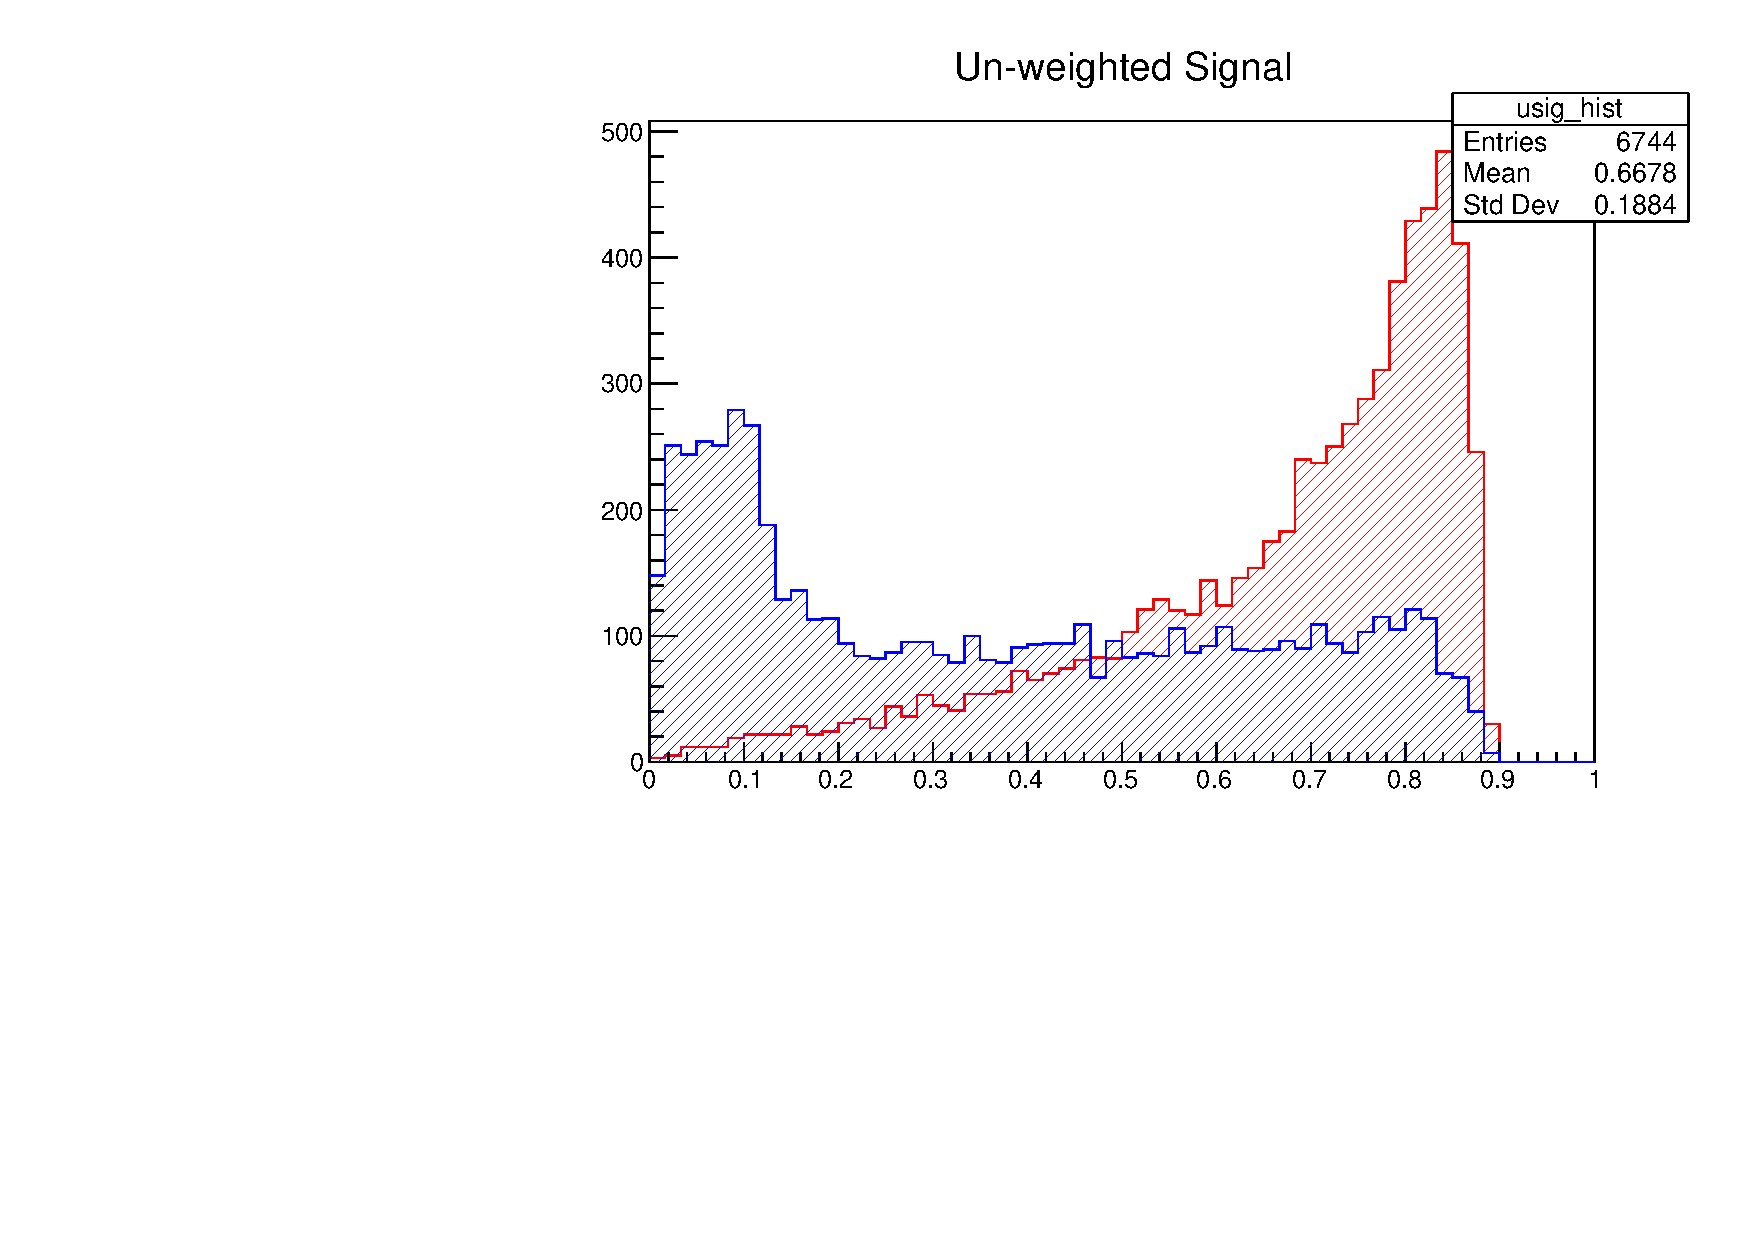
\includegraphics[width=\textwidth]{img/sep}
	      \caption{Distribution of model scores for signal (red) and background (blue) events}
	\end{subfigure}

	\caption{Diagnostic plots for a train ANN with two layers of 7 and 6 hidden nodes }
	\label{fig:label}
\end{figure}